\documentclass[10pt,a4paper]{ivoa}
\usepackage[top=1in, bottom=0.75in, left=0.75in, right=0.75in]{geometry}
\usepackage{hyperref}
\usepackage{parskip}
\input tthdefs
\input gitmeta

\title{ProposalDM: A Data model for Observation Proposals}

% see ivoatexDoc for what group names to use here; use \ivoagroup[IG] for
% interest groups.
\ivoagroup{Data Models}

\author[????URL????]{Paul Harrison}

\editor{Paul Harrison}

% \previousversion[????URL????]{????Concise Document Label????}
\previousversion{This is the first public release}
       

\begin{document}
\begin{abstract}
This document and associated files define a data model in VO-DML that is intended to be suitable for exchanging
    information pertaining to making observation proposals. It is envisaged that the model will be useful in two scenarios.
\begin{itemize}
    \item transferring information between different Observatories' application processes.
    \item observatory scheduling systems being able to automatically extract source lists.
\end{itemize}
\end{abstract}


\section*{Acknowledgments}

Work on this standard is partially funded by the Opticon RadioNet Pilot project within the Horizon2020 programme, contract no. 101004719.

\section*{Conformance-related definitions}

The words ``MUST'', ``SHALL'', ``SHOULD'', ``MAY'', ``RECOMMENDED'', and
``OPTIONAL'' (in upper or lower case) used in this document are to be
interpreted as described in IETF standard RFC2119 \citep{std:RFC2119}.

The \emph{Virtual Observatory (VO)} is a
general term for a collection of federated resources that can be used
to conduct astronomical research, education, and outreach.
The \href{https://www.ivoa.net}{International
Virtual Observatory Alliance (IVOA)} is a global
collaboration of separately funded projects to develop standards and
infrastructure that enable VO applications.


\section{Introduction}


The concept of a common project DM was discussed in \cite{2008SPIE.7019E..0PB}, and whilst this model limits itself to
only the proposal part, the general concept of attempting this level of interoperability is inspired by that paper.

There was a workshop held at ESO \url{https://www.eso.org/sci/meetings/2018/proposal-tools-workshop.html} which reviewed
proposal systems, and this model tries to benefit from the lessons learnt during that workshop.

The detail of the model derives inspiration from two particular sources;
\begin{enumerate}
    \item The data model from the NorthStar tool (TODO cite)
    \item The Alma Project Data model \cite{alma:projdm}.
\end{enumerate}


\subsection{Role within the VO Architecture}

\begin{figure}
\centering

% As of ivoatex 1.2, the architecture diagram is generated by ivoatex in
% SVG; copy ivoatex/archdiag-full.xml to role_diagram.xml and throw out
% all lines not relevant to your standard.
% Notes don't generally need this.  If you don't copy role_diagram.xml,
% you must remove role_diagram.pdf from SOURCES in the Makefile.

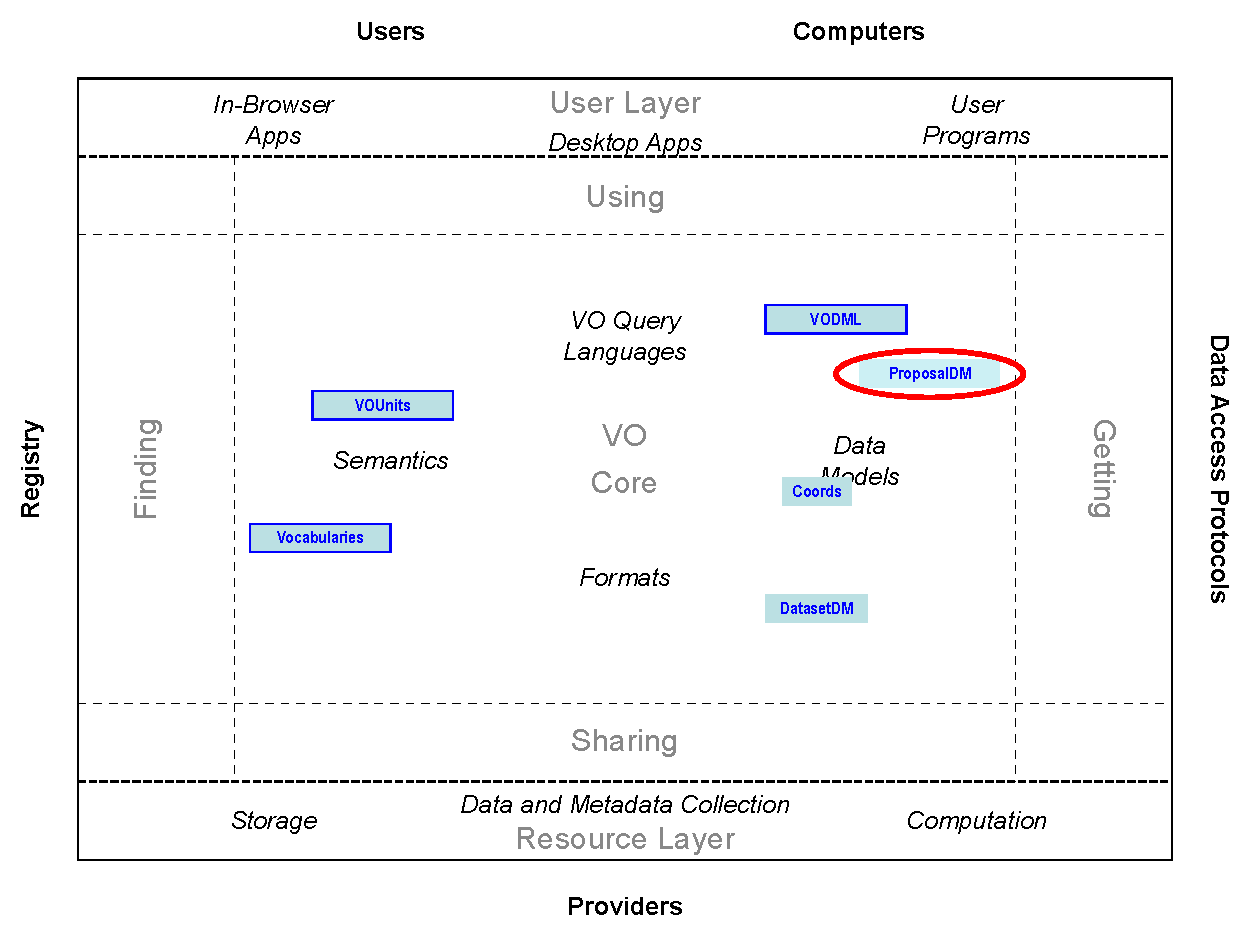
\includegraphics[width=0.9\textwidth]{role_diagram.pdf}
\caption{Architecture diagram for this document}
\label{fig:archdiag}
\end{figure}

Fig.~\ref{fig:archdiag} shows the role this document plays within the
IVOA architecture \citep{2010ivoa.rept.1123A}.


\section{High-level design requirements}

The proposal part model is primarily designed from the proposing astronomer's point-of-view, and does not contain all of the technical detail
that would be necessary from the observatory point-of-view to actually perform detailed instrument set-up for instance, though it does
strive to provide all the information necessary to schedule observations. Some top-level requirements that follow from this approach are;

\begin{enumerate}
    \item The science goal is uppermost
    \begin{itemize}
        \item specify the target objects.
        \item necessary physics goals on the observation.
    \end{itemize}
    \item Specifics of instrumental configuration are not considered - only the broad physics of what the instrument should achieve
\end{enumerate}

In addition there are some other high level requirements of how the review should work that have driven the design;

\begin{enumerate}
    \item It should be easy to reuse the proposal for many observatories.
    \item Proposers should be anonymous to the reviewers (who indeed should be anonymous to the proposers).
\end{enumerate}


The proposal management part of the model adds extra information that the observatory needs to specify what resources are available
and to provide a method of scoring the proposal. This is deliberately created as a separate part of the overall model to help
to enforce the separation in functions so that the same proposal might be more easily submitted to several observatories.

\include{generated/proposaldm.vo-dml_desc}

\begin{figure}
    \centering
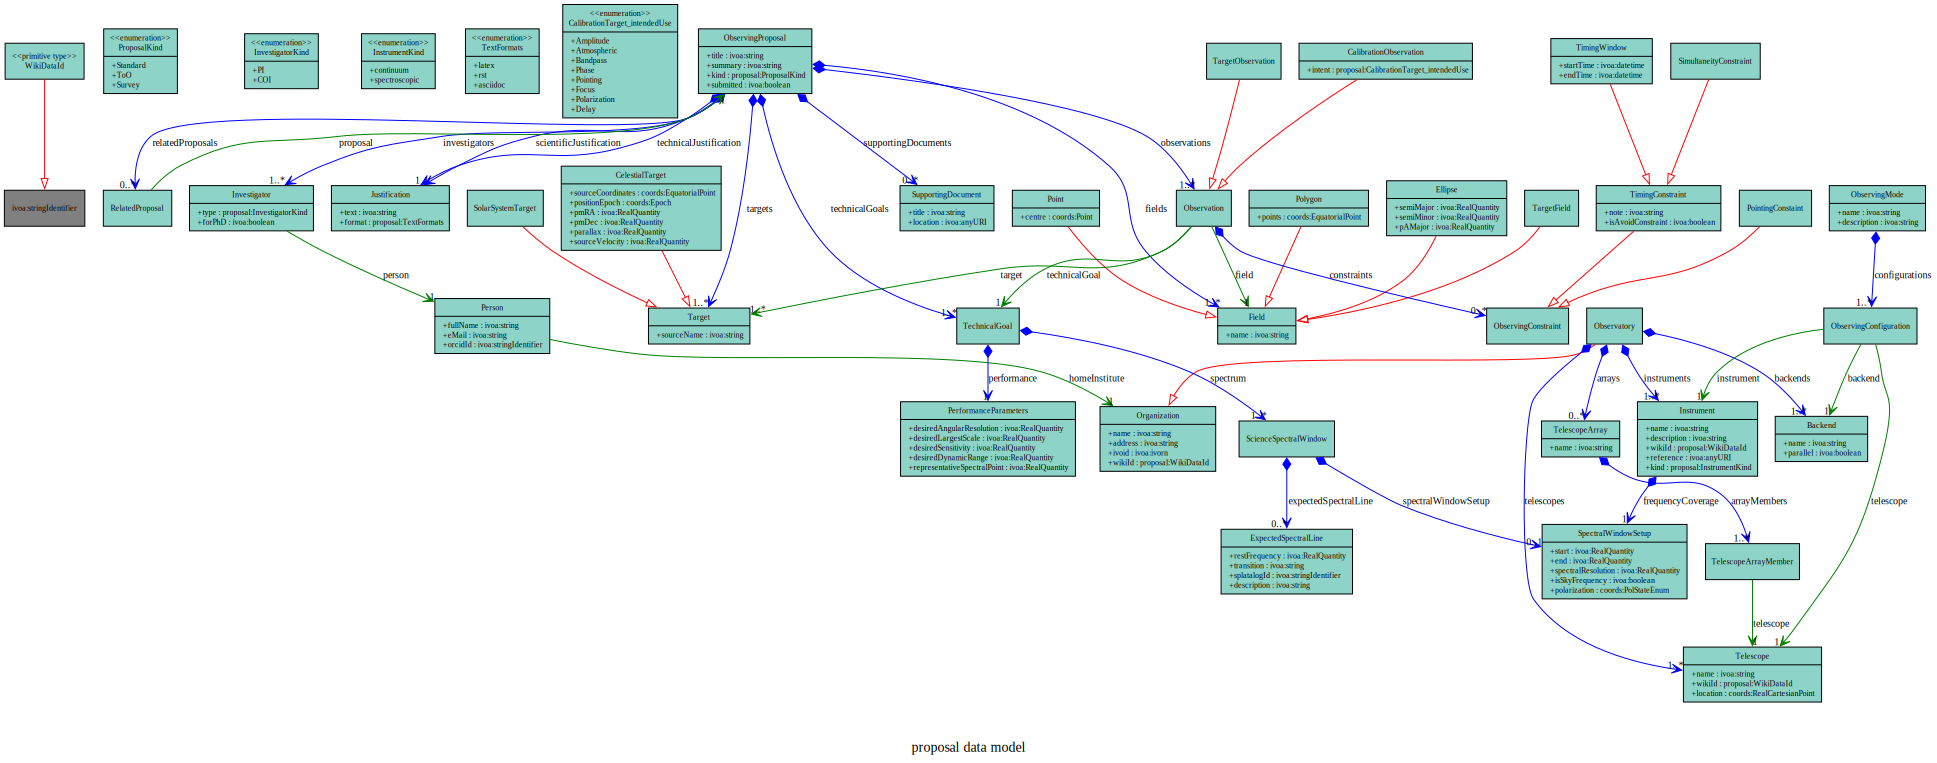
\includegraphics[width=\textwidth]{generated/proposaldm.vo-dml.png}
\caption{The Proposal Data Model}
\label{fig:propdm}
\end{figure}

\include{generated/proposalManagement.vo-dml_desc}
\begin{figure}
    \centering
    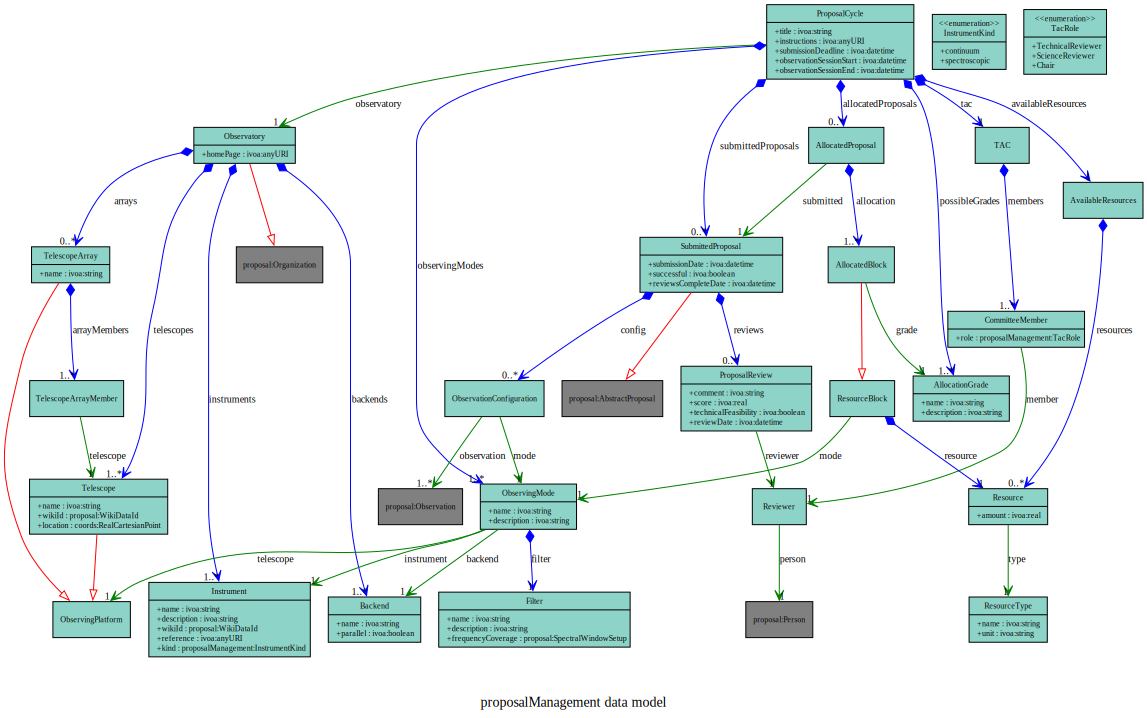
\includegraphics[width=\textwidth]{generated/proposalManagement.vo-dml.png}
    \caption{The Proposal Management Data Model}
    \label{fig:propmdm}
\end{figure}



\appendix
\section{Changes from Previous Versions}

No published versions yet.
% these would be subsections "Changes from v. WD-..."
% Use itemize environments.


% NOTE: IVOA recommendations must be cited from docrepo rather than ivoabib
% (REC entries there are for legacy documents only)
\bibliography{references,ivoatex/ivoabib,ivoatex/docrepo}


\end{document}
